\documentclass[UTF8]{ctexart}
\usepackage{ctex}
\usepackage{geometry}
\usepackage{enumitem}
\usepackage{indentfirst}
\usepackage{color}
\usepackage{fancyhdr}
\usepackage{amsmath}
\usepackage{graphicx}
\usepackage{amssymb}
\usepackage{tikz}
\usepackage{cases}
\usepackage{array}
\usepackage{mathrsfs}
\usepackage{extarrows}
\usepackage{pifont}

% 设置纸张和页边距——A4
\geometry{papersize={21cm,29.7cm}}
\geometry{left=3.18cm,right=3.18cm,top=2.54cm,bottom=2.54cm}

% 一级标题靠左
\CTEXsetup[format={\Large\bfseries}]{section}

% 去除页眉
\pagestyle{plain}

% 开始文档内容
\begin{document}

\title{信号与系统课程笔记:Lecture 28}
\author{授课教师:秦雨潇 \\
        笔记记录:李梦薇}
\date{2023 年 12 月 15 日(第十五周,周五)}
\maketitle

\section{求全响应}
\subsection{零状态}
$y[k]-5y[k-1]+6y[k-2]=f[k]$,$f[k]=4^kU[k]$ \par
\noindent
\begin{flalign*}
  \qquad \text{z域:}Y(z)-5z^{-1}Y(z)+6z^{-2}Y(z)&=F(z) &\\
  (1-5z^{-1}+6z^{-2})Y(z)&=F(z) &\\
  Y(z)&=\frac{z^2}{z^2-5z+6}\cdot F(z) &\\
  \frac{Y(z)}{z}&=\frac{z}{z^2-5z+6}\cdot\frac{z}{z-4} &\\
  \frac{Y(z)}{z}&=\frac{z_1}{z-2}+\frac{z_2}{z-3}+\frac{z_3}{z-4} &\\
  Y(z)&=\frac{z_1z}{z-2}+\frac{z_2z}{z-3}+\frac{z_3z}{z-4} &\\
\end{flalign*} \par
则$y[k]=z_12^kU[k]+z_23^kU[k]+z_34^kU[k]$
\subsection{零输入}
$y[k]-5y[k-1]+6y[k-2]=f[k]$,$f[k]=0$,$y[-1]=a_1$,$y[-2]=a_2$ \par
\noindent
\begin{flalign*}
  \qquad \text{z域:}Y(z)-5(z^{-1}Y(z)+y[-1]z^0)+6(z^{-2}Y(z)+y[-2]z^0+y[-1]z^{-1})&=0 &\\
  (1-5z^{-1}+6z^{-2})Y(z)-(5a_1+6a_2+6a_1z^{-1})&=0 &\\
  \text{(令}5a_1+6a_2=\alpha\text{,}6a_1=\beta\text{)}Y(z)&=\frac{\alpha+\beta z^{-1}}{1-5z^{-1}+6z^{-2}} &\\
  Y(z)&=\frac{\alpha z^2+\beta z}{z^2-5z+6} &\\
  \frac{Y(z)}{z}&=\frac{\alpha z+\beta}{z^2-5z+6} &\\
  \frac{Y(z)}{z}&=\frac{z_1}{z-2}+\frac{z_2}{z-3} &\\
  Y(z)&=\frac{z_1z}{z-2}+\frac{z_2z}{z-3} &\\
\end{flalign*} \par
则$y[k]=z_12^kU[k]+z_23^kU[k]$

\section{z域的系统函数}
$H(Z)\rightleftarrows h[k]$ \par
本质和$H(\omega)$,$H(s)$相同。\par
\subsection{求法}
\begin{enumerate}[label=(\arabic*),itemindent=0pt,labelindent=\parindent,labelwidth=2em,labelsep=5pt,leftmargin=*]
  \item 差分方程
  \item $h[k]\rightarrow H(z)$
  \item $H(z)=\frac{Y(z)}{F(z)}$
\end{enumerate}\par
\subsection{$H(z)$的应用场景}
\begin{enumerate}[label=(\arabic*),itemindent=0pt,labelindent=\parindent,labelwidth=2em,labelsep=5pt,leftmargin=*]
  \item $H(z)\rightarrow h[k]$
  \item $H(z)\rightarrow Y(z)$
  \item $H(z)$和初始状态可以求零输入响应。
  \item $H(z)\rightarrow$系统的差分方程。
  \item 可以画框图和流图。
  \item 可以得到系统的零极图,判断系统的稳定性。
  \item $H(z)\rightarrow$系统的“频率特性”。\par
        例1:某LTI系统,$f[k]=(-0.5)^kU[k]$,$Y_{zs}[k]=[\frac{3}{2}(\frac{1}{2})^k+4(-\frac{1}{3})^k-\frac{2}{9}(-\frac{1}{2})^k]U[k]$,\par
        \begin{itemize}[label=,left=2.25em]
          \item 求$h[k]$和ODE。
          \item \textcircled{1} \ 求$h[k]$:$F(z)=\frac{z}{z+0.5}$
                \begin{itemize}[label=,left=5.2em]
                  \item $Y(z)=\frac{3}{2}\frac{z}{z-\frac{1}{2}}+4\frac{z}{z+\frac{1}{3}}-\frac{9}{2}\frac{z}{z+\frac{1}{2}}$
                  \item $H(z)=\frac{Y(z)}{F(Z)}=\frac{1+2z^{-1}}{1-\frac{1}{6}z^{-1}-\frac{1}{6}z^{-2}}$
                  \item $\cdots$
                \end{itemize}
          \item \textcircled{2} \ 求ODE:$(1-\frac{1}{6}z^{-1}-\frac{1}{6}z^{-2})Y(z)=(1+2z^{-1})F(z)$
                \begin{itemize}[label=,left=5.7em]
                  \item $y[k]-\frac{1}{6}y[k-1]-\frac{1}{6}y[k-2]=f[k]+2f[k-1]$
                \end{itemize}
        \end{itemize}
        例2:\par
        \begin{figure}[h]
          \centering
          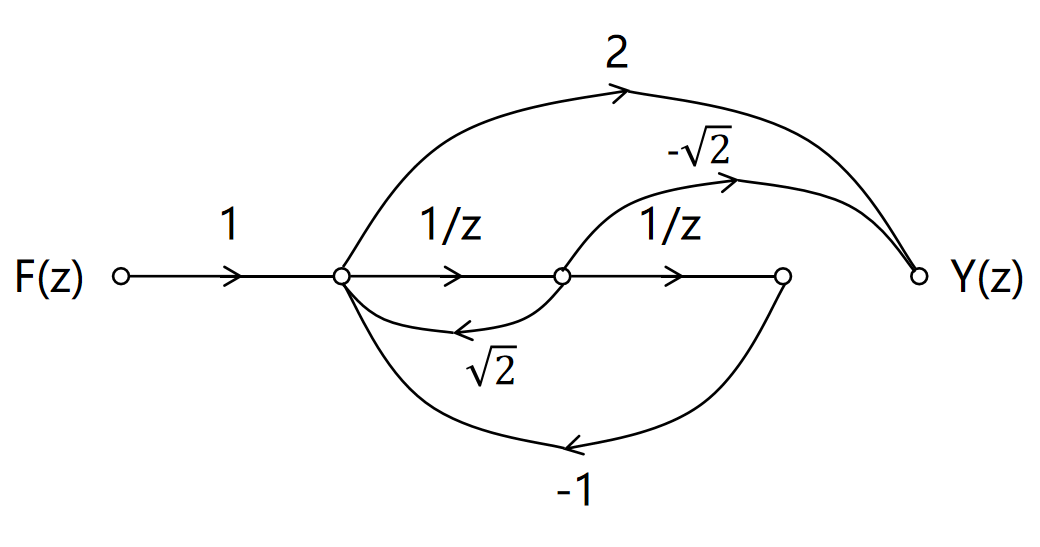
\includegraphics[scale=0.3]{例题2.png}
        \end{figure}
        \begin{itemize}[label=,left=2.25em]
          \item $y[k]-\sqrt{2}y[k-1]+y[k-2]=-\sqrt{2}f[k-1]+2f[k-2]$
        \end{itemize}
\end{enumerate}\par

\section{z域的系统零极图}
$H(z)=\frac{b_m(z-\xi_1)(z-\xi_2)\cdots(z-\xi_m)}{(z-p_1)(z-p_2)\cdots(z-p_n)}$ \par
$\forall\xi_i$,$H(z)\big{|}_{z=\xi_i}=0$称为零点。\par
\hspace*{\fill} \par
总结:\textcircled{1} \ 所有极点在单位圆内,系统稳定。$\quad |a|<1\Leftrightarrow \lim_{k\to+\infty}a^k=0$
\begin{itemize}[label=,left=4.5em]
  \item \textcircled{2} \ 有一个极点在单位圆外,系统不稳定。
  \item \textcircled{3} \ 有极点在单位圆上,“一阶”:“临界稳定”。$\quad1^kU[k]\Leftrightarrow\cos\omega kU[k]$
        \begin{itemize}[label=,left=10.15em]
          \item “二阶或以上”:不稳定。
        \end{itemize}
\end{itemize}

\section{朱利准则}
见课本。

\section{系统稳定性(BIBO,Bounded Input Bounded Output)}
$\sum_{k=0}^{+\infty}|h[k]|<+\infty$(系统稳定的充要条件)\par
极点在单位圆内或$H(z)$的收敛域包含单位圆是判断系统BIBO的充要条件。

\section{系统对正弦(余弦)序列的响应}
$y(t)=e^{j\omega_0t}*h(t)=|H(\omega_0)|e^{j(\omega_0t+\theta)}$,$\theta=\angle{H(\omega_0)}$ \par
\begin{figure}[h]
  \centering
  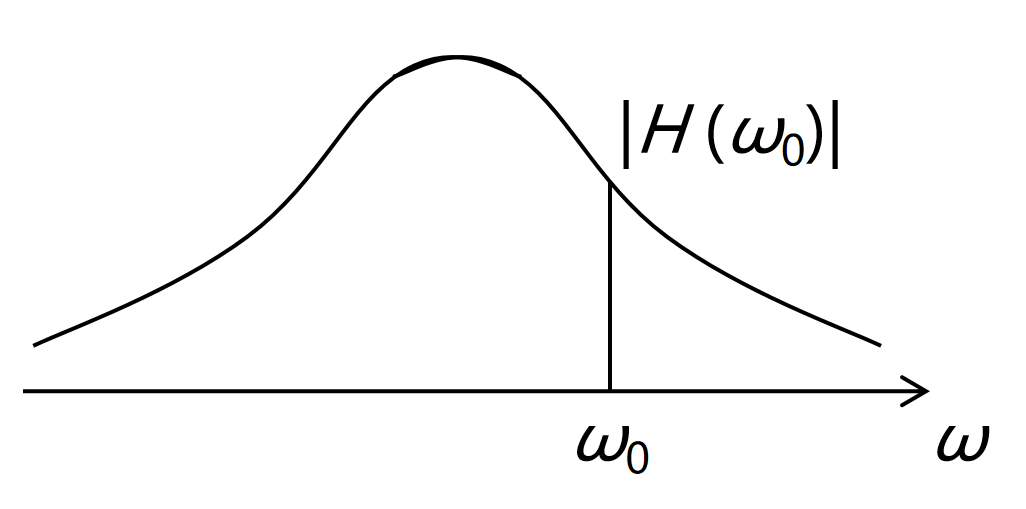
\includegraphics[scale=0.25]{系统对正弦序列的响应.png}
\end{figure}
例题:$H(\omega)=\frac{1-j\omega}{j\omega-0.5}$(或$H(s)=\frac{1-s}{s-0.5}$),$f(t)=10\cos(628Tt+\frac{\pi}{6})$,$T=10^{-3}$s \par
\begin{itemize}[label=,left=4.5em]
  \item $f(t)\rightarrow H(\omega)$(或$H(s)$)$\rightarrow$?
  \item $H(z)=\frac{1-z}{z-0.5}$,$f[k]=10\cos(628Tk+\frac{\pi}{6})$,$T=10^{-3}$s
  \item $f[k]\rightarrow H(z)\rightarrow$?
  \item 解:$H(\omega_0)=H(\omega)\big{|}_{\omega=\omega_0}=\frac{1-e^{j\omega}}{e^{j\omega}-0.5}\big{|}_{\omega=628\times10^{-3}}$
        \begin{itemize}[label=,left=1.5em]
          \item $|H(\omega_0)|=\alpha$,$\angle{H(\omega_0)}=Ae^{j\theta}=\beta$
          \item $y(t)=\alpha10\cos(628Tt+\frac{\pi}{6}+\beta)$
        \end{itemize}
\end{itemize}

\newpage
\section{$H(z)$中零极图的配置}
$|H(z)|=\frac{|\prod_{i=1}^{m}(z-\xi_i)|}{|\prod_{i=1}^{n}(z-p_i)|}$
\begin{figure}[h]
  \centering
  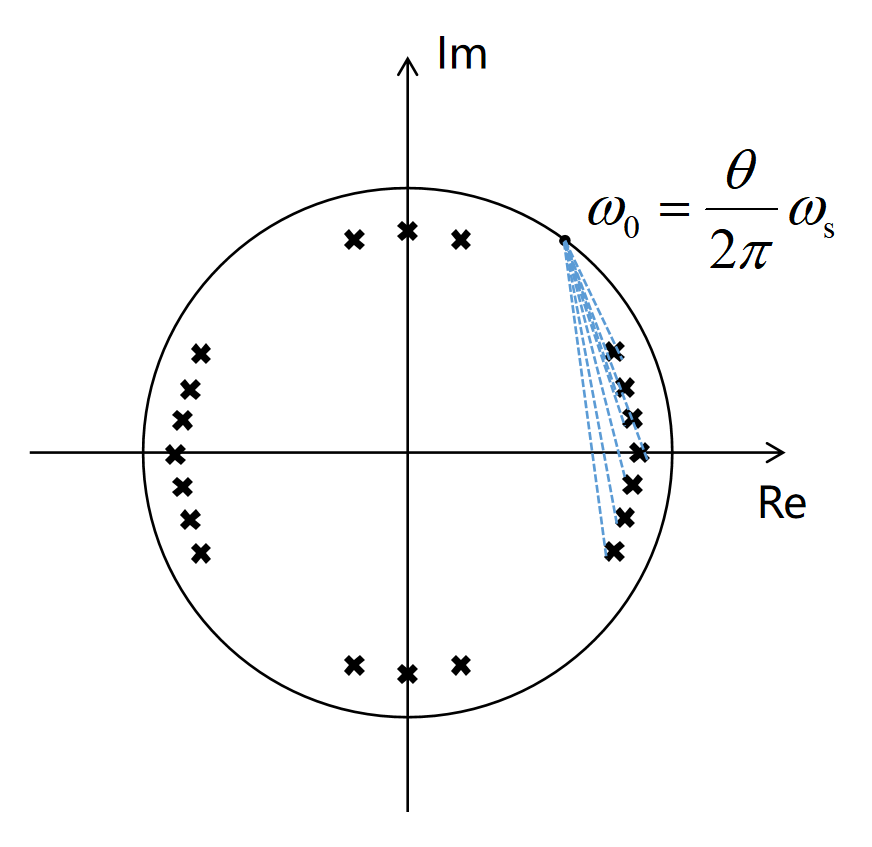
\includegraphics[scale=0.3]{零极图配置.png}
\end{figure}

\end{document}